\PassOptionsToPackage{unicode=true}{hyperref}

% print mode
\documentclass[handout]{beamer}
% presentation mode
%\documentclass{beamer}

\usetheme{Montpellier}
\usepackage[T2A]{fontenc}
\usepackage[utf8x]{inputenc}
\usepackage[russian]{babel}
\usepackage{default}

\usepackage{minted}

\usepackage{fancyvrb}

\usepackage{tikz}
\usetikzlibrary{positioning,arrows,shapes,shadows,calc}

\usepackage{graphicx}

\tikzstyle{file} = [
rounded corners=0.2cm,
thick,
minimum size=1cm,
draw=green!50!black!50,
top color=white,
bottom color=green!50!black!30,
drop shadow
]

\tikzstyle{oldfile} = [
rounded corners=0.2cm,
thick,
dashed,
minimum size=1cm,
draw=green!50!black!50,
top color=white,
bottom color=green!50!black!10,
drop shadow
]

\tikzstyle{commit} = [
%rectangle,
rounded corners=0.2cm,
thick,
minimum size=1cm,
draw=blue!50!black!50,
top color=white,
bottom color=blue!50!black!20,
drop shadow
]

\definecolor{listing}{rgb}{0.95,0.95,0.95}

\title{Системы контроля версий}
\date{}

\begin{document}
\begin{frame}
	\maketitle
\end{frame}

\begin{frame}{Содержание}
	\tableofcontents
\end{frame}

\section{Знакомство с системами контроля версий}

\begin{frame}{Предпосылки создания СКВ}
	\begin{itemize}
		\item{Необходимо хранить историю версий проекта}\pause
		\item{Архивы вида \texttt{001.tgz}, \texttt{002.tgz} и так далее --- непрактично и неудобно}\pause
		\item{Совместная работа над проектом --- ещё сложнее}\pause
		\item{Решение? Системы контроля версий}
	\end{itemize}	
\end{frame}

\begin{frame}{Современные СКВ}
	Виды СКВ:\pause
	\begin{itemize}
		\item{Локальные --- невозможность совместной работы}\pause
		\item{Централизованные (Subversion, CVS) --- сильная зависимость от центрального репозитория}\pause
		\item{Распределённые (Git, Mercurial)}
	\end{itemize}
\end{frame}

\section{Знакомство с Git}

\begin{frame}{Знакомство с Git}
	\begin{itemize}
		\item{Git --- распределённая система контроля версий}\pause
		\item{Подробное руководство: {\color{blue} \url{https://git-scm.com/book/ru/v1}}}\pause
		\item{Создание нового репозитория: \texttt{git~init}}\pause
		\item{Клонирование уже существующего репозитория: \texttt{git~clone}}
	\end{itemize}
\end{frame}

\begin{frame}{Коммиты}
	\begin{tikzpicture}[
	align=center,
	thick,
	node distance=1.7cm,
	text height=1.5ex,
	text depth=.25ex,
	auto
	]
	
	\node (a0) {a.txt:};
	\node[file,right of=a0] (a1) {A1}; 
	\node[oldfile,right of=a1] (a2) {A1};
	\node[oldfile,right of=a2] (a3) {A1};
	\node[file,right of=a3] (a4) {A2};
	
	\node[below of=a0] (b0) {main.c:};
	\node[file,right of=b0] (b1) {B1}; 
	\node[oldfile,right of=b1] (b2) {B1}; 
	\node[file,right of=b2] (b3) {B2}; 
	\node[oldfile,right of=b3] (b4) {B2}; 
	
	\node[below of=b0] (d0) {Makefile:};
	\node[file,right of=d0] (d1) {D1}; 
	\node[file,right of=d1] (d2) {D2}; 
	\node[oldfile,right of=d2] (d3) {D2}; 
	\node[file,right of=d3] (d4) {D3}; 
	
	\node[commit,above of=a1] (c1) {C1};
	\node[commit,right of=c1] (c2) {C2};
	\node[commit,right of=c2] (c3) {C3};
	\node[commit,right of=c3] (c4) {C4};
	
	\path[->] (c1) edge (c2);
	\path[->] (c2) edge (c3);
	\path[->] (c3) edge (c4);
	\end{tikzpicture}
\end{frame}

\begin{frame}{Состояния файлов в репозитории}
	\begin{center}
		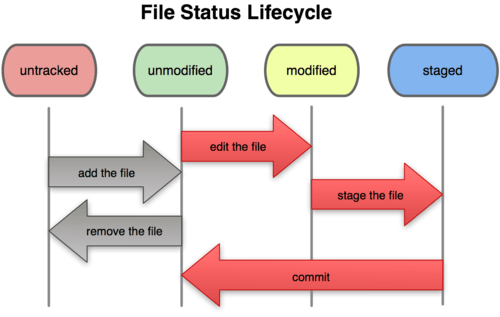
\includegraphics[width=8cm]{files/vcs/file_lifecycle.png}
		
		{\color{gray}\tiny Источник картинки: \color{blue}\url{https://git-scm.com/book/ru/v1/}\color{gray}, раздел 2.2}
	\end{center}
\end{frame}

\begin{frame}
	\begin{itemize}
		\item{Для того, чтобы загрузить последнюю версию проекта, нужно выполнить команду \texttt{git pull}. Вообще, во избежание конфликтов версий при командной работе над проектом следует делать это всякий раз перед началом работы.}\pause
		\item{Чтобы загрузить изменения в репозиторий, нужно выполнить несколько операций. Во-первых, git даёт возможность пользователю хранить <<лишние>> файлы в каталоге с проектом (например, конфигурационные файлы IDE или логи). Кроме того, какие-то важные файлы могли быть случайно удалены, переименованы или изменены.}\pause
		\item{Поэтому про \emph{все} полезные изменения нужно сообщить git с помощью команды \texttt{git add <file1> <file2> ...} (вместо файлов можно указывать каталоги; если нужно добавить все изменения, можно применить команду \texttt{git add .}, находясь в корневом каталоге проекта)}
	\end{itemize}
\end{frame}

\begin{frame}
	\begin{itemize}
		\item{Чтобы увидеть, какие файлы нуждаются в индексировании и какие изменились по сравнению с предыдущей версией, или \emph{коммитом}, как это принято называть в git, воспользуйтесь командой \texttt{git status}}\pause
		\item{Чтобы увидеть разницу между теми файлами, которые реально есть в рабочем каталоге, и файлами в индексе git, выполните команду \texttt{git diff}. Добавление ключа \texttt{-{}-staged} или \texttt{-{}-cached} позволит увидеть разницу между проиндексированными изменениями и последним коммитом}\pause
		\item{Наконец, когда все нужные изменения проиндексированы, нужно все эти изменения зафиксировать. Делается это с помощью команды \texttt{git commit}. При этом откроется текстовый редактор, в котором нужно написать некоторое пояснение к коммиту. Чтобы избедать этого, можно выполнить коммит с ключом \texttt{-m}: \texttt{git commit -m "Msg"}}
	\end{itemize}
\end{frame}

\begin{frame}
	\begin{itemize}
		\item{Для синхронизации с удалённым репозиторием нужно воспользоваться командой \texttt{git push}. Будьте готовы к тому, что у Вас попросят пароль, если, конечно, не настроена аутентификация по ключу}\pause
		\item{}
	\end{itemize}
\end{frame}

\end{document}
